\section{Introduction to Data Analysis: Data Classification}
\label{sec:data_analysis}

\subsection{Supervised Classification}
\textcolor{blue}{\textbf{Question 1:}}
\textit{Enumerate main supervized classification techniques and describe them in few lines.}

%~~~~~~~~~~~~~~ANSWER~~~~~~~~~~~~~~
Supervised Classification is... ???

Some typical Supervised Classification techniques are listed and described below:
\begin{enumerate}
    \item \textbf{k-Nearest Neighbours (k-NN):} The most simple classification algorithm where the principle is to find the \textit{k} closest data in the dataset to determine its class. 
    First a distance has to be defined, which is not always easy.

    
    \item \textbf{Maximum Likelihood:} A simple classifier based on the probability distribution.
    It assumes the data follows a known probability distribution (typically normal or Gaussian distr.) for each class.
    ML estimates the probability that a given data point belongs to each possible class and assigns it to the class with the highest likelihood.

    \begin{equation*}
        C^* = \underset{C_i}{\operatorname{argmax}} \, P(C_i \mid o)
    \end{equation*}

    
    \item Bayesian Classification:
    Based on the bayesian rule where given an observation \textit{o}, the \textit{prior} (a priori probability), is described as:
    \begin{equation*}
        P(C_i \mid o) = \frac{P(o \mid C_i) P(C_i)}{P(o)}
    \end{equation*}
    where $P(C_i \mid o)$ is called \textit{posterior} (a posterior probability).

    More text??

    
    \item \textbf{Linear Classification:}
    The most simple classification rule, where the objective is to establish a hyperplane, \textit{HP}, that separates the data into two groups:
    \begin{equation*}
    \begin{split}
        &\mathcal{H} : w_0 + \vec{w} \cdot \vec{x} = 0 \\
        &\text{In a \textit{n}-D space:} \\
        &\mathcal{H} : w_0 + w_1 x_1 + w_2 x_2 + \cdots + w_n x_n = 0
    \end{split}
    \end{equation*}

    Linear Classification is only possible if the data is \textit{linearly separable}. If not, there are infinite solutions
    An example of Linear Classification is the Perceptron Algorithm, which bla bla
    
    
    \item Neural Networks:
    \item Decision Trees:
    \item Concept Lattices:
    \item Support Vector Machine
    \item Random Forests:
    \item etc.
\end{enumerate}



\textcolor{blue}{\textbf{Question 2:}}
\textit{Apply and compare the following algorithms:
\begin{enumerate}
    \item 1-NN (your programme)
    \item Neural Network    
\end{enumerate}
on 'Spain Beach' image or another of your choice}

\begin{enumerate}
    \item 1-NN 

    The first step is to select the data for our classes, which we select at random in predefined areas for 'land', 'beach', 'foam' and 'ocean' classes.
    \begin{figure}[!ht]
        \centering
        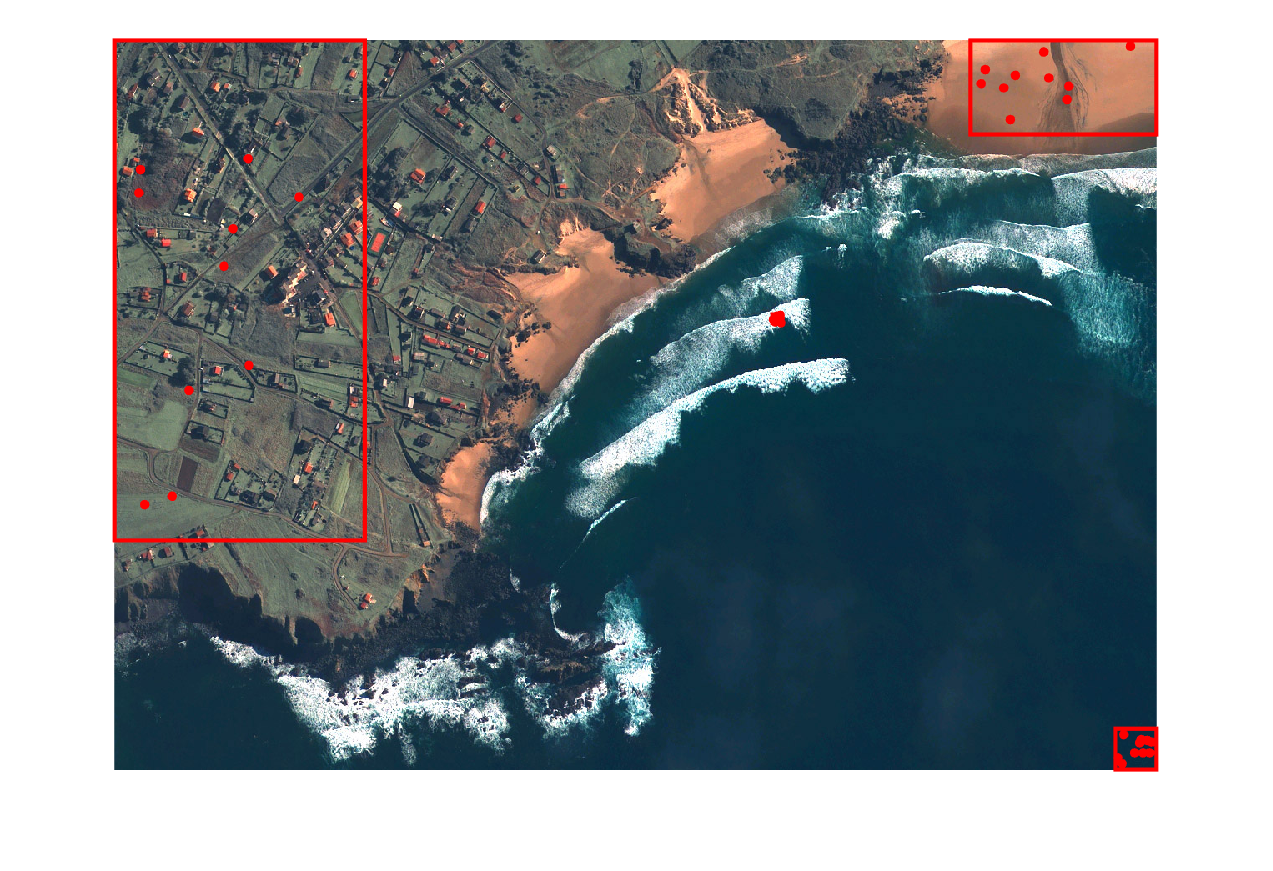
\includegraphics[width=0.45\linewidth]{Doc/Graphics/Part4/kNN_training_sets.png}
        \caption{Randomly selected training data}
    \end{figure}

    The output of the algorithm gives us the beach we want to extract
    \begin{figure}[!ht]
        \centering
        \begin{subfigure}{0.45\textwidth}
            \centering
            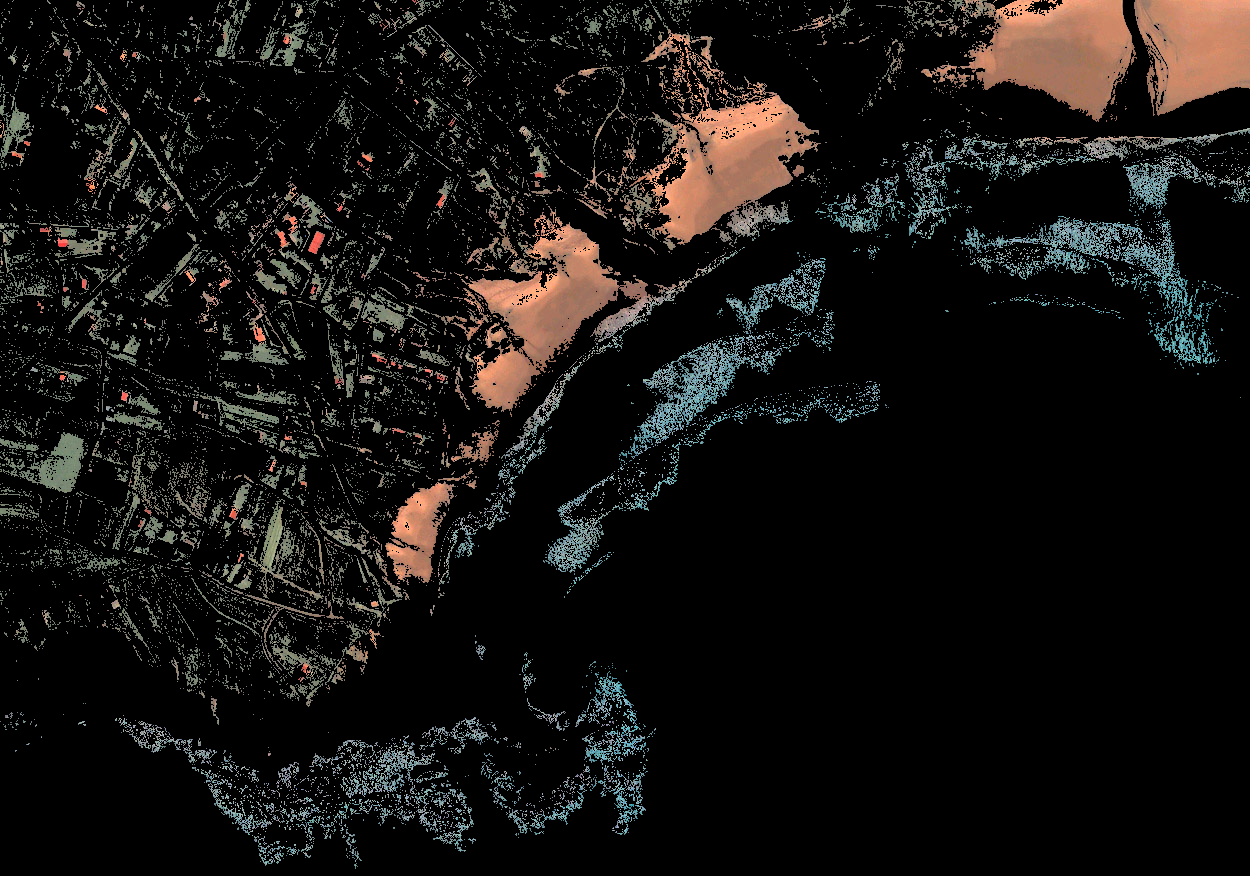
\includegraphics[width=\textwidth]{Doc/Graphics/Part4/kNN_classified_beach.png}
            \caption{Raw output}
        \end{subfigure} \hfill
        \begin{subfigure}{0.45\textwidth}
            \centering
            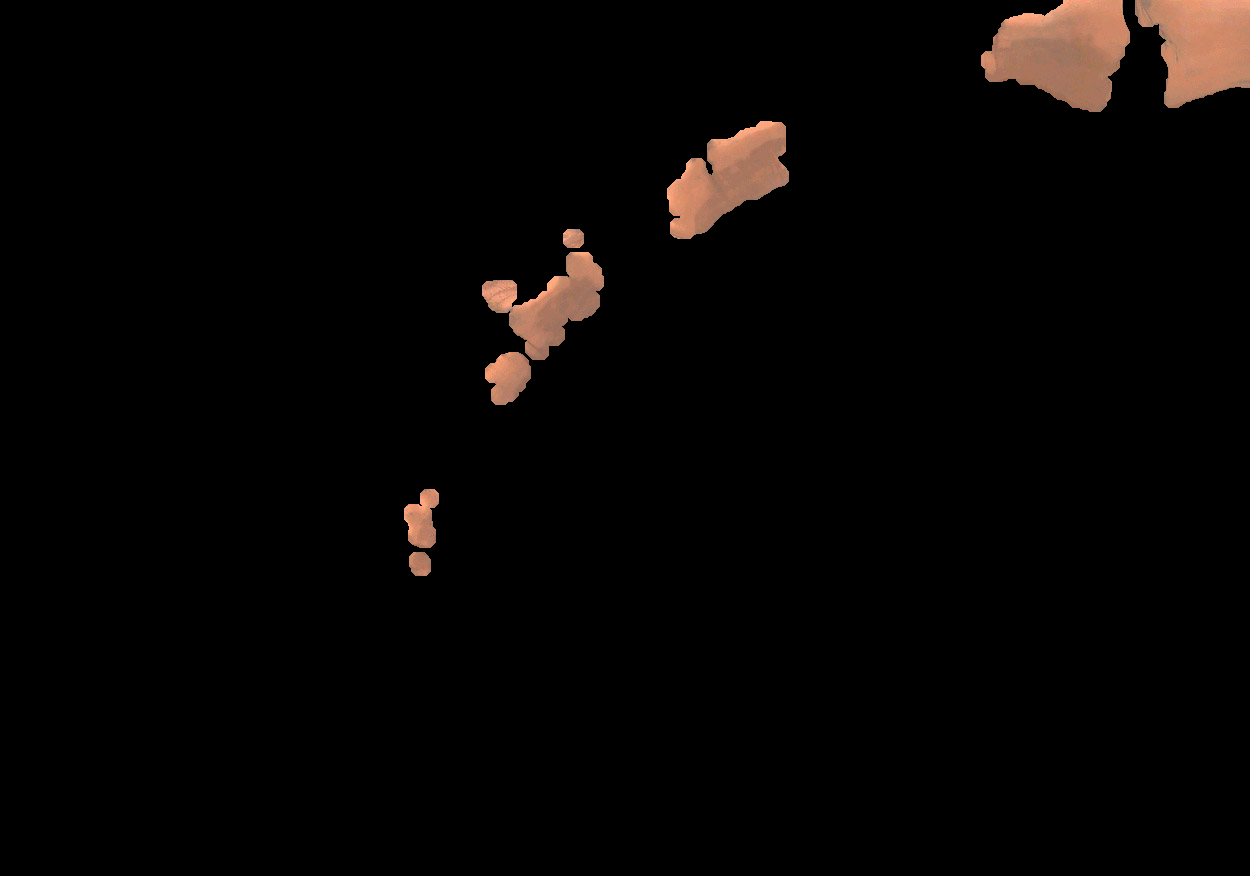
\includegraphics[width=\textwidth]{Doc/Graphics/Part4/kNN_masked_beach.png}
            \caption{Smoothened output}
        \end{subfigure}
        \caption{Extracted beach}
        \label{fig:enter-label}
    \end{figure}  
    \FloatBarrier
    
    \item Neural Network
    
    We select two sets of training data, which gives us two classes: 'beach' and 'not beach'. 
    \begin{figure}[!ht]
        \centering
        \begin{subfigure}{0.2\textwidth}
            \centering
            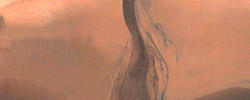
\includegraphics[width=\textwidth, angle=90]{Doc/Graphics/Part4/training_set_beach.png}
            \caption{Beach}
        \end{subfigure}
        \begin{subfigure}{0.4\textwidth}
            \centering
            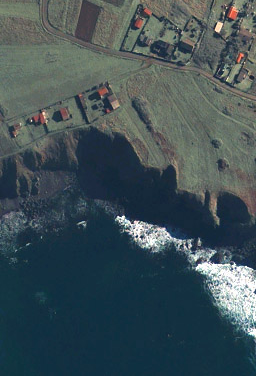
\includegraphics[width=0.5\textwidth, angle=90]{Doc/Graphics/Part4/training_set_other.png}
            \caption{Not beach}
        \end{subfigure}
        \caption{Training sets}
    \end{figure}
    \FloatBarrier

    The target assigned to beach RGB values is 1 and 0 for the rest. Training the network goes smoothly, and its output results in the following extraction of the beach:
    \begin{figure}[!ht]
        \centering
        \begin{subfigure}{0.45\textwidth}
            \centering
            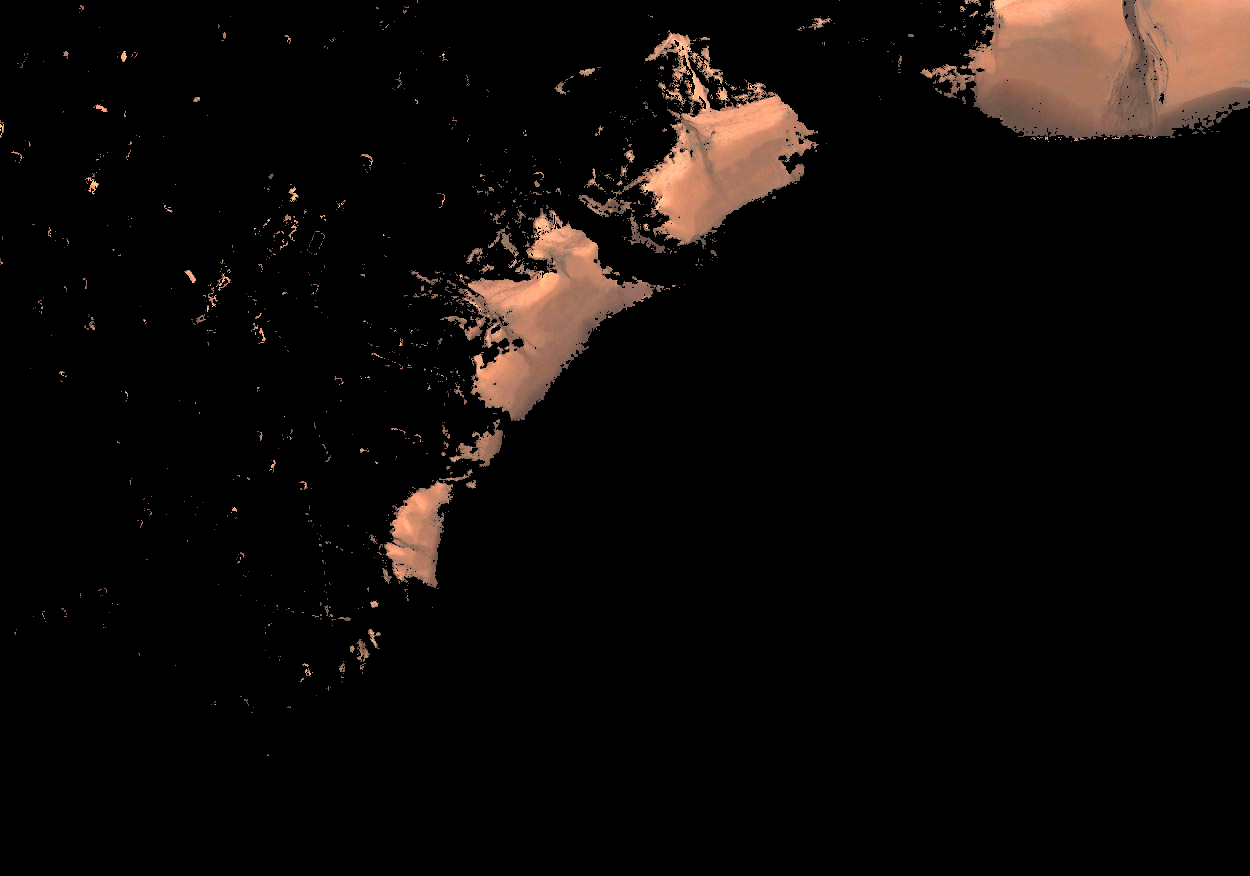
\includegraphics[width=\textwidth]{Doc/Graphics/Part4/nn_classified_beach.png}
            \caption{Raw output}
        \end{subfigure} \hfill
        \begin{subfigure}{0.45\textwidth}
            \centering
            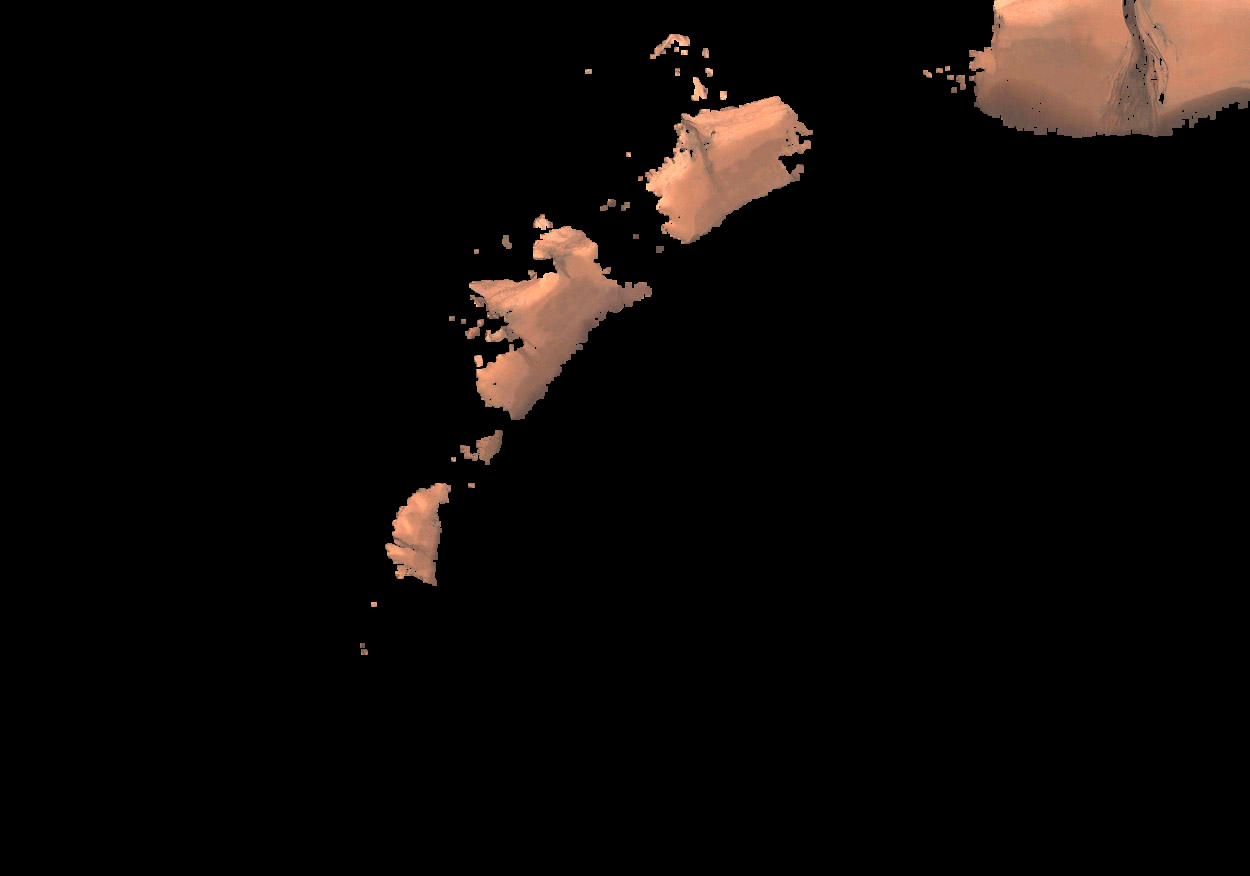
\includegraphics[width=\textwidth]{Doc/Graphics/Part4/nn_masked_beach.png}
            \caption{Smoothened output}
        \end{subfigure}
        \caption{Extracted beach}
        \label{fig:enter-label}
    \end{figure}
    \FloatBarrier

    \item Comparison

    There are two noticeable differences: speed and noise level. The neural network is much more performant in terms of speed and produces an output with much less noise and better classification (like the river delta in the top right corner).
\end{enumerate}



\textcolor{blue}{\textbf{Question 3:}}
\textit{Search on internet one of the two the following algorithms and apply it to the same image
\begin{enumerate}
    \item SVM
    \item Ramdom Forest
\end{enumerate}
}




\subsection{Unsupervised Classification}
\textcolor{blue}{\textbf{Question 4:}}
\textit{Enumerate main unsupervized classification techniques and describe them in few lines.}


\textcolor{blue}{\textbf{Question 5:}}
\textit{Apply the following algorithms with the dedicated objective
\begin{enumerate}
    \item k-means algorithm to define the four classes automatically and speed-up the classification process
    \item Pseudo-Inverse technique to estimate the position of a planet
    \item PCA technique to reduce the size of an image
\end{enumerate}
}